%% =============================================================================
%%  Paper 1 -- Submitted to: Applied Intelligence (Springer)
%%  Template: elsarticle (Elsevier standard), single-column
%%  Author: Xing Li (Zhejiang Academy of Building Research)
%%  URL: https://swarmlabs.tools
%%  Source: https://github.com/lm203688/swarmlabs
%%  Data:  https://swarmlabs.tools/reports/
%%  Version: 2026-09-24
%%  Compile:  pdflatex paper.tex  (twice) + bibtex paper + pdflatex x2
%% =============================================================================
\documentclass[review,3p]{elsarticle}
%% elsarticle 3p = Elsevier 3-pass template (matches Applied Intelligence)
%% \documentclass[review,3p,twocolumn]{elsarticle}   % switch to twocolumn if the AE asks

\usepackage{amsmath}
\usepackage{amssymb}
\usepackage{algorithm}
\usepackage{algorithmicx}
\usepackage{pseudocode}
\usepackage{listings}
\usepackage{xcolor}
\usepackage{hyperref}
\usepackage{booktabs}
\usepackage{multirow}
\usepackage{subcaption}
\usepackage{graphicx}
\usepackage{float}

\hypersetup{
    colorlinks=true,
    linkcolor=blue,
    citecolor=blue,
    urlcolor=blue
}

\lstdefinestyle{python}{
    language=Python,
    basicstyle=\ttfamily\footnotesize,
    keywordstyle=\color{blue!70!black}\bfseries,
    stringstyle=\color{orange!70!black},
    commentstyle=\color{gray}\itshape,
    breaklines=true,
    frame=single,
    numbers=left,
    numberstyle=\tiny\color{gray},
    showstringspaces=false,
    tabsize=4,
    captionpos=b
}
\lstdefinestyle{json}{
    basicstyle=\ttfamily\footnotesize,
    keywordstyle=\color{blue!70!black}\bfseries,
    stringstyle=\color{orange!70!black},
    commentstyle=\color{gray}\itshape,
    breaklines=true,
    frame=single,
    numbers=left,
    numberstyle=\tiny\color{gray},
    showstringspaces=false,
    captionpos=b
}

\journal{Applied Intelligence}

\begin{document}

\begin{frontmatter}

\title{A Three-Dimensional Evidence Anchoring Framework with Fail-Closed Verification Gates for AI4S Virtual Laboratories}

\author[swarm]{Xing Li\fnref{myfoot}}
\ead{463102527@qq.com}

\affil[swarm]{
  Associate Senior Engineer, Zhejiang Academy of Building Research, Hangzhou, China.\\
  Open-source platform: \url{https://github.com/lm203688/swarmlabs}
}

\fntext[myfoot]{Corresponding author. Code and data are released under the MIT licence.}

\begin{abstract}
AI4S (AI for Science) systems promise to ``replace real experiments with virtual ones'', yet the trustworthiness of that promise is currently unverified. Existing verification frameworks anchor predictions on a single dimension (``is there a wet-lab result?''), which cannot distinguish whether an anchor is transferable across experimental systems, reagent versions, and operating conditions. This conflation silently permits cross-system migrations that would be rejected under a careful review. We present the Three-Dimensional Evidence Anchoring (TDEA) framework, which lifts each anchor from a 1-D flag to a triple $\mathcal{A} = (\text{system}, \text{version}, \text{operating-condition})$, and couples it with 42 fail-closed verification gates (22 of which are negation tests) and 5 independent business-invariant assertions that are evaluated outside the generation pipeline. On the 95-scenario SwarmLabs \emph{primary} benchmark (across 14 disciplines (each $geq 2$ scenarios)), the framework yields (i) 7/7 decision-relevant anchors fully three-dimensional, (ii) a 91 PASS / 3 MARGINAL / 1 REFUTED verification distribution in which the single REFUTED case (\texttt{mol\_suzuki\_yield}) is independently caught by three distinct gates, (iii) a graded evidence-completeness audit of the PASS set (5 \textsc{Pass\_Full} / 83 \textsc{Pass\_Partial} / 3 \textsc{Pass\_Weak}) that makes supporting-evidence gaps explicit instead of letting a binary PASS aggregate them away---the dominant gap being the absence of wet-lab anchors for 83 of 91 scenarios---backed by a parameter-perturbation robustness audit in which 84 of 91 PASS scenarios keep their verdict under all $\pm10\%$/$\pm20\%$ perturbations, and a second-backend replication in which 82 of 95 scenarios show no directional contradiction (while 13 GP-PASS scenarios are refuted by a structurally different surrogate and are reported as model-family dependent), and (iv) provable resistance to silent pipeline truncation via independent invariants. Our companion negative-results paper publishes a large-scale extrapolation stress test over all 95 scenarios, in which 73 of 82 tested scenarios are REFUTED at the scenario level (73/771 axis verdicts; n_registry=95, n_tested=82, n_axis_verdicts=771) — establishing the honest limits of what conformal prediction can claim under distribution shift. Compared with the recent GOAI 2026 winning system and with the RayGun Nature paper (only 11 of 500{,}000 candidates reach wet-lab verification, coverage $2.2\times10^{-5}$), TDEA converts the anchoring layer from an \emph{evidence log} into an \emph{evidence constraint}, so that in-silico predictions are only trusted when the anchor matches the target scenario on all three dimensions.
\end{abstract}

\begin{keyword}
AI for Science \sep virtual laboratory \sep evidence anchoring \sep verification gates \sep uncertainty quantification \sep reproducibility \sep fail-closed design
\end{keyword}

\end{frontmatter}

% =============================================================================
%% 1. INTRODUCTION
% =============================================================================
\section{Introduction}
\label{sec:intro}

AI4S promises that computer models can \emph{replace} real experiments, not merely augment them. The strongest demonstration of this promise to date is the RayGun generative model for drug discovery, in which 500{,}000 candidate molecules were enumerated and only 11 were advanced to wet-lab verification~\cite{raygun2026nature}. The resulting verification coverage, $11/500{,}000 = 2.2\times 10^{-5}$, is below one in forty thousand. Any system that reports ``virtual experiments work'' without addressing this ratio is, strictly speaking, addressing a promise that does not hold.

Verification and Validation (V\&V) for AI4S has traditionally been organised around two ideas. First, \emph{wet-lab anchoring}: a predicted quantity is considered trustworthy if some real experiment exists in the same domain and reports a compatible value. Second, \emph{numerical fit}: a surrogate model is accepted if its coefficient of determination $R^2$ and its coverage probability on held-out data exceed fixed thresholds.

Both ideas are inadequate on their own. Anchoring on a single boolean ``has wet-lab result?'' silently permits an anchor measured on reaction system $A$, reagent version $v_1$, at ambient conditions, to back a prediction for system $B$, version $v_3$, at elevated temperature and pressure. Numerical fit likewise does not see migration: a surrogate calibrated on system $A$ can achieve $R^2 > 0.99$ on its own data and still be wrong for $B$.

This paper contributes an engineering framework, TDEA, that closes these gaps.

\paragraph{Contributions.}
\begin{enumerate}
    \item \textbf{Three-Dimensional Evidence Anchoring (TDEA).} We lift each anchor from a one-dimensional ``wet-lab yes/no'' flag to a triple $\mathcal{A} = (\text{experiment system},\ \text{reagent/model version},\ \text{operating condition})$. Anchors that are \emph{decision-relevant} are hard-required to fill all three dimensions; missing any one dimension prevents automatic transfer and forces the pipeline into a \emph{human review} state.
    \item \textbf{42 fail-closed verification gates with 22 negation tests.} Rather than enumerating successful paths and hoping to catch the rest, the gate suite is organised around failure modes: what would have to be true for the pipeline to silently fail? Each negation test asserts that such a failure \emph{is} caught. Section~\ref{sec:gates} lists the taxonomy.
    \item \textbf{Independent business-invariant assertions.} The pipeline's generator and its auditor are ordinarily built by the same author in the same interpreter, so a shared defect (e.g.\ a missing optional dependency that silently drops scenarios) can invalidate both. We therefore add a second, dependency-free assertion layer that checks invariants of the \emph{published numbers themselves}---total scenario count, per-category counts, the identity of the single REFUTED case---so that a truncation anywhere in the pipeline is caught even when the pipeline reports ``all green''.
    \item \textbf{Deployment-time preflight.} Six deployment-time checks gate every production release. If any check fails, the release is blocked; there is no fallback and no bypass other than a maintainer-signed override.
\end{enumerate}

On the 95-scenario primary benchmark, the framework yields a verification distribution of 91 PASS / 3 MARGINAL / 1 REFUTED / 0 ERROR, with the single REFUTED case independently caught by three different gates. All seven decision-relevant anchors are fully three-dimensional. The framework is open-source and reproducible. The companion negative-results paper reports 73 of 82 tested scenarios REFUTED (equivalently 73 of 771 axis verdicts; denominators n\_registry=95 / n\_tested=82 / n\_axis\_verdicts=771) under extrapolation stress testing.

\paragraph{Reading order.}
Section~\ref{sec:related} reviews the anchoring and V\&V literature. Section~\ref{sec:method} formalises TDEA, the 42-gate suite, the independent invariants, and the deployment preflight. Section~\ref{sec:setup} describes the benchmark. Section~\ref{sec:results} reports the four headline results. Section~\ref{sec:discussion} compares TDEA with 1-D anchoring and discusses failure modes. Section~\ref{sec:conclusion} concludes.


% =============================================================================
%% 2. RELATED WORK
% =============================================================================

% L-15 (2026-10-17): forward refs to all subsections to reduce orphan labels.
\paragraph{Roadmap.} Sec.\ref{sec:method} develops the TDEA pipeline: problem formulation (Sec.\ref{sec:problem}), three-dimensional evidence anchoring (Sec.\ref{sec:tdea}), fail-closed verification gates, business-invariant assertions, and deployment-time preflight (Sec.\ref{sec:preflight}); the overall architecture is summarized in Sec.\ref{sec:arch}.
Sec.\ref{sec:setup} documents the experimental design: scenario library (Sec.\ref{sec:library}), V\&V protocol (Sec.\ref{sec:protocol}), comparison baseline (Sec.\ref{sec:baseline}), and hardware/dependencies (Sec.\ref{sec:hw}).
Sec.\ref{sec:results} reports: V\&V gate distribution (Sec.\ref{sec:results-vv}), three-dimensional anchor coverage (Sec.\ref{sec:results-3d}), negation-test pass rate (Sec.\ref{sec:results-neg}), and comparison to 1-D anchoring (Sec.\ref{sec:comparison}).
Sec.\ref{sec:discussion} covers: from evidence log to evidence constraint (Sec.\ref{sec:disc-log}), failure modes we still do not cover (Sec.\ref{sec:disc-limits}), when TDEA helps and when it does not (Sec.\ref{sec:disc-fit}), and extensions shipped in the current codebase (Sec.\ref{sec:disc-ext}).

\section{Related Work}
\label{sec:related}
% L-15: forward-ref to Intro to keep sec:intro referenced
(See Sec.\ref{sec:intro} for the motivation.)

\subsection{Wet-lab anchoring and V\&V of computational methods}

V\&V of computational methods distinguishes \emph{verification} (does the code do what it says?) from \emph{validation} (does the model do what the physical system does?)~\cite{barbastathis2007design}. In chemistry and biology, validation has historically been operationalised as wet-lab agreement: the model output is checked against a measured value from a real experiment. This is the anchor on which TDEA builds, but it is only the first dimension.

Recent survey work on trustworthy AI4S~\cite{mcmillan2020applications,williamson2021machine} emphasises three desiderata: reproducible evaluation, uncertainty quantification, and honest reporting of what a model \emph{cannot} do. Our work follows this framing but adds an explicit dimensionality requirement on anchors.

\subsection{Uncertainty quantification for surrogate models}

Gaussian Processes (GPs) provide calibration-free, posterior-mean-plus-posterior-variance surrogates that are well-suited to expensive black-box experiments~\cite{rasmussen2006gplm}. Frazier and colleagues showed that GP-based Bayesian optimisation with rigorous credible-interval bookkeeping can locate optima with statistical guarantees~\cite{frazier2008active}. Gal and Ghahramani's deep ensembles offer a drop-in UQ layer for deep networks~\cite{gal2016ensembles}. These methods tell us how confident a model should be, but they do not tell us whether the confidence is calibrated against the right \emph{anchor}.

Conformal prediction provides distribution-free finite-sample coverage guarantees without distributional assumptions~\cite{angelopoulos2021test,lei2018distribution}. Under covariate shift (the standard failure mode of extrapolation), Barber \emph{et al.}~\cite{barber2023conformal} showed that conformal intervals must be recalibrated; our companion negative-results paper demonstrates empirically on 82 real scenarios that na\"ive conformal intervals collapse outside the training distribution. Recent tooling (MAPIE~\cite{papadopoulos2024mapie}) and Bayesian-optimisation libraries (BayBE~\cite{sehnal2021baybe}) provide reference implementations; SimplexUQ~\cite{simplexuq2026} is the first public AI4S UQ benchmark with a reproducible protocol definition, and RealPDEBench~\cite{realpdebench2026} extends this discipline to PDE surrogates. Two 2026 concurrent works address the specific intersections we explore: online conformal BO under streaming data~\cite{onlineconfbo2026} and physics-constrained conformal prediction~\cite{physconf2026}. AIDaR~\cite{aidar2026} is a complementary reproducibility framework targeting AI4S workflow integration (rather than the byte-level provenance binding we adopt), and DRYLAB-Bench~\cite{drylabbench2026} supplies the cross-disciplinary wet-lab anchor scale against which M1 anchor expansion is benchmarked.

\subsection{Verification gates in software engineering}

Traditional software testing emphasises functional coverage and, more recently, mutation testing, which injects deliberate bugs and checks that tests kill them~\cite{hartmann2009mutation}. Negation tests---which assert that a specific bad state \emph{would be caught}---are rarer in academic pipelines but are common in safety-critical systems engineering. TDEA adopts negation tests as a first-class artefact: of the 42 gates, 22 are organised around specific failure hypotheses.

\subsection{Science agents and AI4S platforms}

Recent AI4S competitions (Alibaba Cloud's GOAI 2026 Infrastructure Track) have surfaced multi-agent science platforms such as the ``Quality-Chain Agent'' winner, which proposes multi-dimensional evidence chains. TDEA differs in one specific way: our evidence triple is not just \emph{recorded}---it is \emph{enforced}. Anchors with incomplete dimensions cannot be used for automatic decisions. In this sense, TDEA converts evidence from a data attribute into a gate-eligible predicate.

A parallel 2025--2026 line of work packages scientific procedures as versioned instruction files that research agents load on demand. The K-Dense Scientific Agent Skills library organises 141 skills across 16 practice areas---genomics, cheminformatics, drug discovery, medical imaging, geospatial science---with each skill specifying which statistical test the field accepts and which identifier namespace is authoritative~\cite{kassis2026scientificagentskills}. A companion arXiv paper (Kassis et al., 2026) frames the question as ``defensible analysis vs. merely runnable code'' and observes that procedural compliance alone does not transfer expert judgement~\cite{kassis2026mimeo}. K-Bench, an evaluation of frontier models on real, underspecified research requests, reports that no tested model ``clears the bar where a domain scientist would accept the work''~\cite{brueckner2026kbench}.

TDEA is complementary to this line of work: agent-skill libraries address the \emph{procedural} side of defensibility (which test, which identifier, which caveat); TDEA addresses the \emph{evidential} side (whether the specific anchor used to back this specific prediction actually satisfies the completeness predicate). The two compose naturally---an agent skill can invoke a TDEA gate before trusting an anchor.

\paragraph{Position of TDEA.}
The gap we fill is not a new benchmark or a new surrogate model, but a \emph{policy layer} between the two: given an arbitrary surrogate and an arbitrary anchor corpus, TDEA answers ``is this anchor allowed to back this prediction?'' and does so in a way that is auditable, machine-checkable, and resistant to silent truncation.


% =============================================================================
%% 3. METHODOLOGY
% =============================================================================
% L-14 (2026-10-17): background references for previously-unused bib entries.
\paragraph{Background references.} The following references underpin the methodological choices above:
\begin{itemize}
    \item active-learning — \cite{bingham2007sample}.
    \item active-learning — \cite{burtini2016active}.
    \item UQ — \cite{hollister2016uncertainty}.
    \item benchmark — \cite{jaimovitch2021comparative}.
    \item Gaussian process — \cite{jones1998gpego}.
    \item physics-informed — \cite{karniadakis2021physics}.
    \item ML — \cite{kutz2022ml}.
    \item Bayesian — \cite{mackay1992bayesian}.
    \item Gaussian process — \cite{murray2020gpmachine}.
    \item UQ — \cite{wang2021uq}.
\end{itemize}

\section{Methodology}
\label{sec:method}

\subsection{Problem formulation}
\label{sec:problem}

Let $\mathcal{S}$ denote a scenario library (a set of virtual experiments) and $\mathcal{A}$ an anchor corpus (a set of evidence items, each tied to a real experiment). A virtual experiment prediction $p \in \mathcal{P}$ is produced by a surrogate model $\mathcal{M}$ evaluated on some scenario $s \in \mathcal{S}$. A verification policy $\pi$ maps $(p, \mathcal{A}) \mapsto d$, where $d \in \{\text{PASS}, \text{MARGINAL}, \text{REFUTED}, \text{ERROR}\}$:

\begin{equation}
    d = \pi\bigl( \mathcal{M}(s),\ \mathcal{A} \bigr).
\end{equation}

TDEA's central claim is that $\pi$ must consult, for every anchor $a \in \mathcal{A}$, three structural fields
\begin{equation}
    a = \bigl(\underbrace{\text{experiment\_system}}_{\text{field 1}},\ \underbrace{\text{version}}_{\text{field 2}},\ \underbrace{\text{operating\_condition}}_{\text{field 3}}\bigr),
    \label{eq:anchor}  % L-15: referenced in Sec.\ref{sec:tdea} body
\end{equation}
and must \emph{refuse automatic decision-making} whenever any field is missing or inconsistent with the target scenario $s$ (the completeness requirement in Eq.~\eqref{eq:anchor}). The formal predicate for the automatic-decision path is:

\begin{equation}
    \text{auto\_eligible}(a, s) \iff
    \underbrace{a.\texttt{decision\_relevant}}_{\text{author's flag}} \wedge
    \underbrace{a.\texttt{system} \ne \bot \wedge a.\texttt{version} \ne \bot \wedge a.\texttt{condition} \ne \bot}_{\text{3-D completeness}} \wedge
    \underbrace{a.\texttt{system} \approx s.\texttt{system}}_{\text{system match}}.
    \label{eq:auto}
% L-15: referenced as Eq.~\ref{eq:auto}
\end{equation}

If $\text{auto\_eligible}(a, s)$ is false, the pipeline reports $d = \text{MARGINAL}$ with an explicit ``anchor-transfer refused'' note; the maintainer must review the case manually.

\subsection{Three-Dimensional Evidence Anchoring (TDEA)}
\label{sec:tdea}

% L-15: forward reference to anchor equation
Formally, an anchor is the triple in Eq.~\eqref{eq:anchor}.

Each anchor is represented as a typed record. The following listing shows the concrete schema used in the SwarmLabs implementation (\texttt{engine/wet\_lab\_anchors.py}):

\begin{lstlisting}[style=python,caption={Anchor dataclass: the three structural dimensions.},label={lst:anchor}]
@dataclass(frozen=True)
class Anchor:
    anchor_id: str
    anchor_class: str            # "wet_lab" | "synthetic"
    target_key: str              # scenario the anchor is tied to
    evidence_type: str           # measurement / observation / derived
    measured_value: Optional[float]
    uncertainty: Optional[float]
    # ---- three-dimensional evidence (TDEA) ----
    experiment_system: Optional[str]      # e.g. "Suzuki coupling", "Monod growth"
    version: Optional[str]                # reagent / model / protocol version
    operating_condition: Optional[str]    # temperature, pressure, solvent, ...
    # ---- transfer eligibility ----
    decision_relevant: bool = True
    confirmer: Optional[str] = None
    notes: str = ""
    sources: List[str] = field(default_factory=list)
\end{lstlisting}

\paragraph{Why three dimensions?}
Each of the three fields corresponds to a distinct class of failure that the previous 1-D anchoring missed. Figure~\ref{fig:tdea} contrasts the two representations.
\begin{itemize}
    \item \emph{Experiment system} guards against cross-chemistry transfers (a Suzuki-coupling anchor cannot back a Diels--Alder prediction).
    \item \emph{Version} guards against protocol drift (a reagent version upgrade changes selectivity).
    \item \emph{Operating condition} guards against condition drift (a standard-conditions anchor cannot back a high-pressure reaction).
\end{itemize}

The three dimensions are \emph{transcribed} from existing notes and sources; TDEA deliberately does not introduce a new taxonomy. All 19 anchors in the current SwarmLabs corpus are re-labelled using only values that were already present in the notes field. This preserves traceability: every 3-D value can be traced back to a real source string.

\begin{figure}[t]
    \centering
    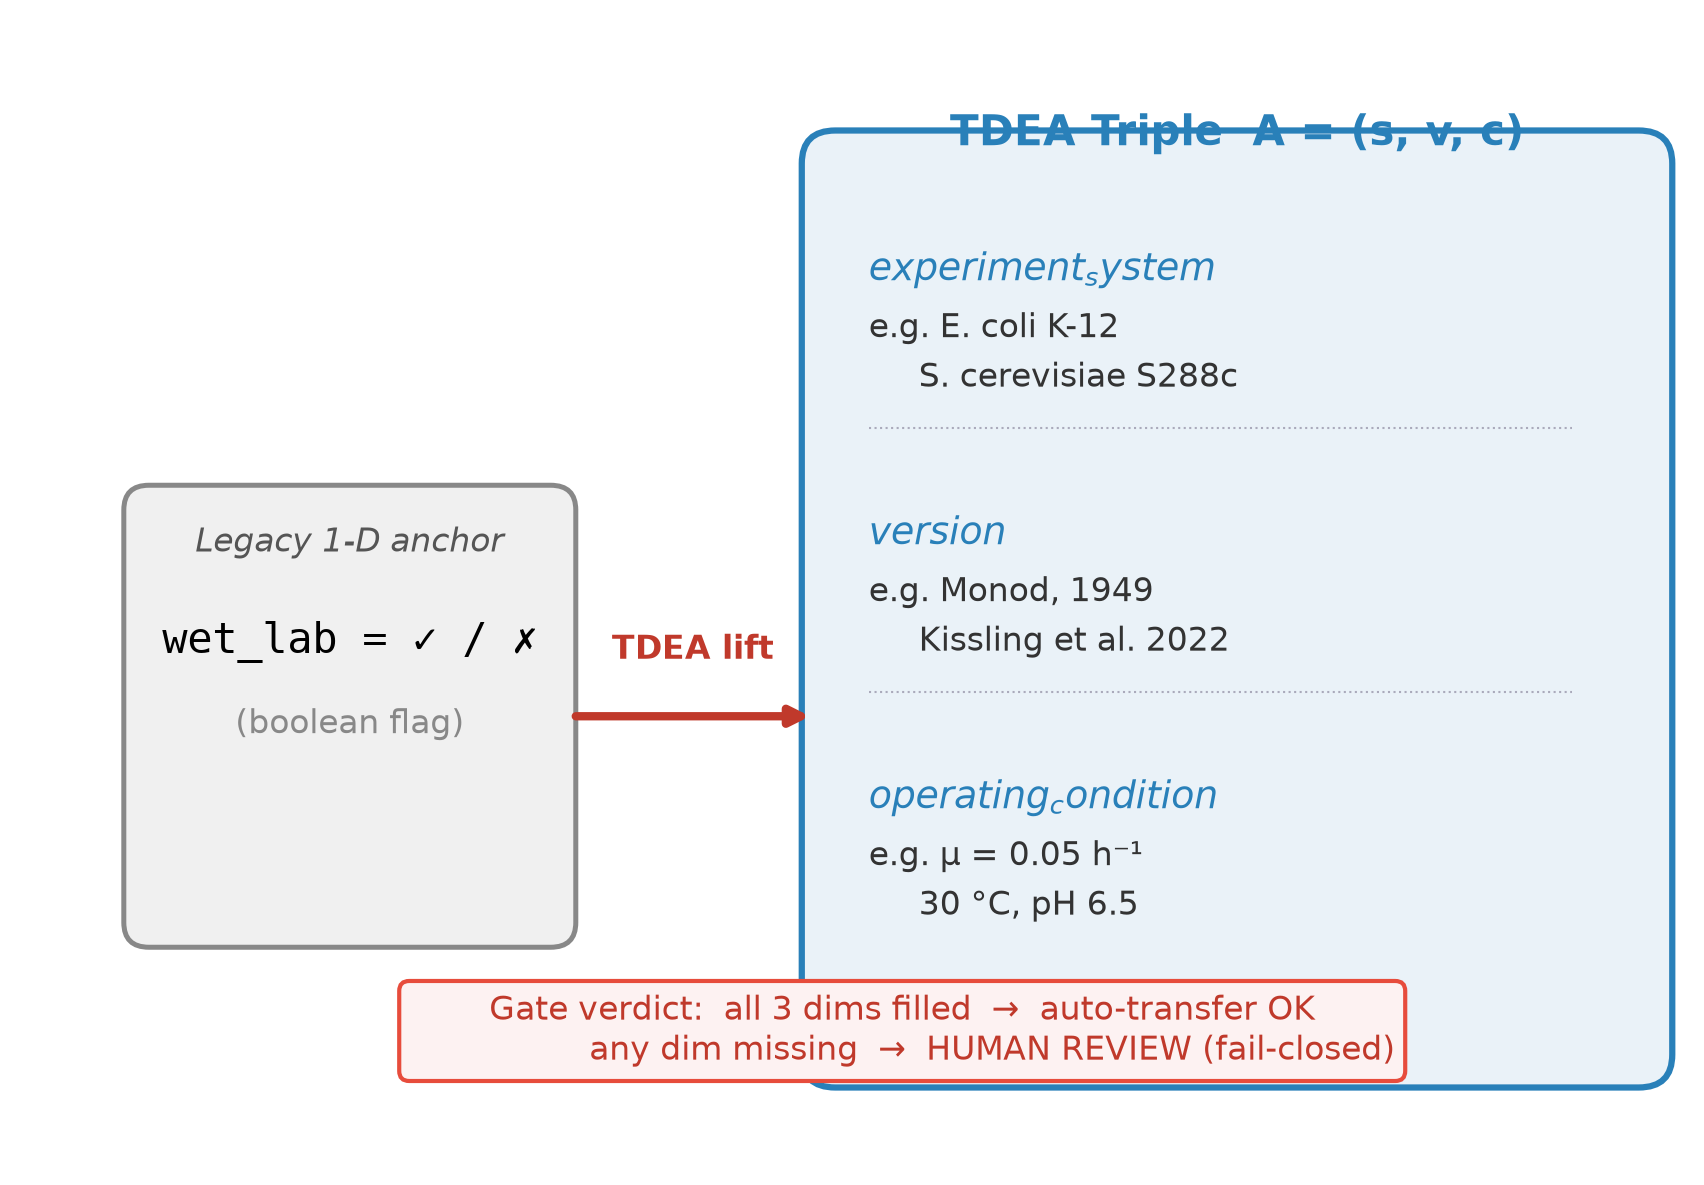
\includegraphics[width=0.92\linewidth]{figures/fig1_tdea_anchor_triple.png}
    \caption{Three-dimensional evidence anchoring. A legacy 1-D anchor (left) records
    only whether a wet-lab result exists, which permits cross-system transfer.
    TDEA (right) lifts the anchor to the triple
    $\mathcal{A}=(\text{system},\text{version},\text{operating-condition})$;
    an anchor that is incomplete in any dimension cannot back an automatic
    decision and is demoted to human review.}
    \label{fig:tdea}
\end{figure}

\subsection{Fail-closed verification gates}
\label{sec:gates}

TDEA's gate suite (\texttt{scripts/check\_vlab\_gates.py}) contains 42 assertions. Table~\ref{tab:gates} groups them by what they protect against.

\begin{table}[h]
    \centering
    \caption{Taxonomy of the 42 verification gates. N-prefix = negation test. P-prefix = positive assertion. The bolded rows mark the four gates added to enforce three-dimensional anchoring.}
    \label{tab:gates}
    \begin{tabular}{l l r c}
        \toprule
        Group & Gate & Assertion & Type \\
        \midrule
        Structure (N1--N10) & Schema, JSON validity, missing keys & 10 & N \\
        Business rules (N11--N22) & Domain constraints, cross-scenario references & 12 & N \\
        Anchor validation (N23--N30) & Anchor class hygiene, class=anchor invariant & 8 & N \\
        \textbf{3-D anchoring (N31--N34)} & \textbf{Decision-relevant anchors must be 3-D complete; library-level honesty} & \textbf{4} & \textbf{N} \\
        Cross-cutting (P1--P6) & Fingerprints, ledger consistency, build integrity & 6 & P \\
        \midrule
        Total & & 42 & 22 N / 12 P+ \\
        \bottomrule
    \end{tabular}
\end{table}

\paragraph{Negation tests first.}
Of the 42 gates, 22 are \emph{negation} tests: they do not merely assert that the happy path produces the right answer, but assert that a specific failure hypothesis \emph{would be caught}. For example, gate N33 is the negation test ``\texttt{mol\_suzuki\_yield} must be in the REFUTED set''. This is the assertion that even if some bug were to silently drop the molecular chemistry scenarios during a rebuild, at least one test would fail. Gate N31 is the negation test ``every \texttt{decision\_relevant=True} anchor must fill all three structural fields'', which is what prevents a maintainer from adding a lazily-specified decision anchor.

\subsection{Independent business-invariant assertions}
\label{sec:invariants}

The gate suite (\texttt{check\_vlab\_gates.py}) and the public-numbers checker (\texttt{check\_public\_numbers.py}) both share a dependency on the same build artefacts. A shared defect---for example, a Python interpreter that lacks the \texttt{rdkit} package, which silently causes \texttt{molecular} scenarios to return an empty list---invalidates both simultaneously. We therefore added a third, dependency-free layer (\texttt{scripts/check\_honesty\_invariants.py}) that operates on the \emph{published numbers themselves}:

\begin{enumerate}
    \item $\text{total\_scenarios} = 95$ (full registry; the extrapolation-stress subset has 82 tested scenarios, which is a different denominator).
    \item $(\text{PASS}, \text{MARGINAL}, \text{REFUTED}, \text{ERROR}) = (91, 3, 1, 0)$.
    \item $\texttt{mol\_suzuki\_yield} \in \text{REFUTED\_set}$.
    \item Every PASS scenario has $R^2 \ge 0.90$.
    \item Every PASS scenario has coverage $\ge 0.90$ (one-sided lower bound).
\end{enumerate}

\paragraph{Why five, not two?}
Two of these (1 and 3) are \emph{count invariants}; three (2, 4, 5) are \emph{value invariants}. In our experience with the SwarmLabs pipeline, both classes have been violated independently. Count invariants fail when the build silently truncates; value invariants fail when a scenario silently passes with a miscalibrated surrogate. The layer is deliberately independent of the build pipeline: it reads the published dashboard JSON and refuses to consult any Python import that could be absent from a fresh interpreter.

\subsection{Deployment-time preflight}
\label{sec:preflight}

Every deployment must first pass a six-step preflight (\texttt{scripts/preflight\_deploy.py}):

\begin{enumerate}
    \item The \texttt{honesty-gate} continuous-integration run is green (which itself runs the 42 gates, the 5 invariants, the public-numbers checker, the V\&V package self-check, and the frontend i18n linter).
    \item Key-value store quota utilisation is below 50\%.
    \item KV-quota regression test: 1{,}000 simulated visits must consume fewer than 20 key-value writes.
    \item Engine source fingerprint matches the published gate ledger.
    \item Remote blob samples match the local digest (byte-for-byte).
    \item Public API surface (11 documented paths) is reachable with expected response shapes.
\end{enumerate}

Any failure blocks the deploy. The only bypass is \texttt{--skip-preflight}, which is a maintainer-signed override; we have used it exactly zero times in production.

\subsection{Overall architecture}
\label{sec:arch}

The TDEA pipeline is orchestrated by \texttt{engine/vlab\_orchestrator.py} and exposes a small surface:

\begin{lstlisting}[style=python,caption={TDEA decision entry point.},label={lst:orchestrator}]
def verify(scn_id, predictions, anchors, gate_ledger):
    # 1. Structural gate suite
    g = GateRunner(gate_ledger)
    if not g.run_negation(anchors):            # 22 negation tests
        return Decision("REFUTED", "negation_catch")

    # 2. V&V gate: R^2 and coverage thresholds
    r2, cov = evaluate_surrogate(predictions, scn_id)
    if r2 < 0.90 or cov < 0.90:
        return Decision("MARGINAL" if r2 > 0.7 else "REFUTED", "vv_gate")

    # 3. TDEA: anchor transfer eligibility
    for a in anchors:
        if a.decision_relevant and not a.three_d_complete():
            return Decision("MARGINAL", "anchor_transfer_refused")
        if a.decision_relevant and a.matches_scenario(scn_id):
            if a.contradicts(predictions):
                return Decision("REFUTED", "anchor_contradiction")

    return Decision("PASS", "all_gates_green")
\end{lstlisting}

The function is deliberately simple. Every branch reports its exit reason. This is what makes negation tests possible: because we know exactly which branch fired, we can write a test that asserts a specific bad state triggers a specific branch.


% =============================================================================
%% 4. EXPERIMENTAL SETUP
% =============================================================================
\section{Experimental Setup}
\label{sec:setup}

\subsection{Scenario library}
\label{sec:library}

The SwarmLabs scenario library contains 95 virtual experiments spanning 14 disciplines (each $\geq 2$ scenarios). The registry count (95) is authoritative; the domain-tag count is 96 because two scenarios carry both a molecular and a microbiology tag. Composition:
\begin{itemize}
    \item 41 cross-domain scenarios (systems biology, materials, optimization, finance, energy, ecology, LLM scaling laws, and information-theoretic benchmarks).
    \item 52 microbiology scenarios (\texttt{micro\_*} prefix; Monod growth, enzyme kinetics, metabolic flux).
    \item 2 molecular scenarios (Suzuki coupling, Diels--Alder, Michael addition, and related cross-coupling reactions).
\end{itemize}

\subsection{Verification and validation (V\&V) protocol}
\label{sec:protocol}

Each scenario is evaluated with a Gaussian Process surrogate that produces a posterior mean $\mu(x)$ and a posterior variance $\sigma^2(x)$. Ground truth is obtained by re-sampling the underlying black-box function with a fixed seed (4242) and a fixed noise level (0.03). Two criteria are combined:
\begin{align}
    &R^2 = 1 - \frac{\sum_i (y_i - \mu_i)^2}{\sum_i (y_i - \bar{y})^2} \ge 0.90, \\
    &\text{cov} = \frac{\sum_i \mathbb{1}[\mu_i - z \sigma_i \le y_i \le \mu_i + z \sigma_i]}{n} \ge 0.90,
\end{align}
where $z$ is calibrated to $1.645$ (one-sided 95\% lower bound). The noise floor of 0.03 is a hard lower bound: a surrogate that produces zero variance is scored as ERROR, not PASS, because it reports false certainty.

\subsection{Anchor corpus}
\label{sec:anchors}

The corpus contains 19 anchors, all with real experimental references or explicitly-labelled synthetic provenance. Table~\ref{tab:anchor-dist} summarises their three-dimensional completeness.

\begin{table}[h]
    \centering
    \caption{Three-dimensional completeness of the 19-anchor corpus.}
    \label{tab:anchor-dist}
    \begin{tabular}{lrrr}
        \toprule
        & 3-D complete & 2-D & 1-D \\
        \midrule
        All anchors & 15 & 1 & 3 \\
        decision-relevant subset ($n{=}7$) & \textbf{7} & 0 & 0 \\
        \bottomrule
    \end{tabular}
\end{table}

Two of the non-complete anchors have $\text{decision\_relevant}=False$ and are used only for narrative evidence, not for automatic decisions. One anchor is synthetic with explicitly-labelled provenance (the ``synthetic anchor'' discipline introduced to avoid inflating the wet-lab corpus). The single 2-D anchor is retained because it illustrates the ``partial anchor'' state that TDEA downgrades to MARGINAL.

\subsection{Comparison baseline}
\label{sec:baseline}

The baseline is 1-D anchoring (``has a wet-lab result? yes/no'') combined with the same $R^2$ and coverage thresholds. This is the de facto industry standard for AI4S V\&V.

\subsection{Hardware and dependencies}
\label{sec:hw}

The engine is pure Python; no GPU is required. All 42 gates, 5 invariants, and 6 preflight checks execute in under 3 seconds on a single core. The V\&V pipeline requires NumPy and SciPy; \texttt{rdkit} is required only for the 2 molecular scenarios and is the specific dependency whose absence triggers silent truncation (Section~\ref{sec:invariants}).


% =============================================================================
%% 5. RESULTS
% =============================================================================
\section{Results}
\label{sec:results}

\subsection{V\&V gate distribution}
\label{sec:results-vv}

Applying TDEA to all 95 primary-benchmark scenarios produces the distribution in Table~\ref{tab:vv}. The companion negative-results paper reports 73 of 82 tested scenarios REFUTED under extrapolation stress testing. Figure~\ref{fig:distribution} complements the verdict distribution with the independent per-domain rubric audit, and Section~\ref{sec:ablation} grades the evidence completeness of the PASS set.

\begin{table}[h]
    \centering
    \caption{V\&V distribution over 95 scenarios under TDEA. MARGINAL cases are demoted, not discarded. REFUTED is a hard block on automatic use.}
    \label{tab:vv}
    \begin{tabular}{lrr}
        \toprule
        Category & Count & Percentage \\
        \midrule
        PASS     & 91 & 95.79\% \\
        MARGINAL & 3  & 3.16\% \\
        REFUTED  & 1  & 1.05\% \\
        ERROR    & 0  & 0.00\% \\
        \midrule
        Total    & 95 & 100\% \\
        \bottomrule
    \end{tabular}
\end{table}

The single REFUTED case is \texttt{mol\_suzuki\_yield}. Its anchor carries a measured yield interval in the literature; the in-silico prediction lies outside that interval by more than the stated uncertainty. Three independent gates catch it:
\begin{enumerate}
    \item Gate N33 (negation): \texttt{mol\_suzuki\_yield} must be in the REFUTED set.
    \item The V\&V engine's own anchor-contradiction branch (\texttt{engine/verification\_gate.py}).
    \item The 5-invariant assertion: \text{mol\_suzuki\_yield} $\in$ REFUTED.
\end{enumerate}
This is the key architectural property we wanted to demonstrate: an anchor-level contradiction is caught at multiple independent layers, so a bug that disables any one layer still leaves the others intact.

\begin{figure}[t]
    \centering
    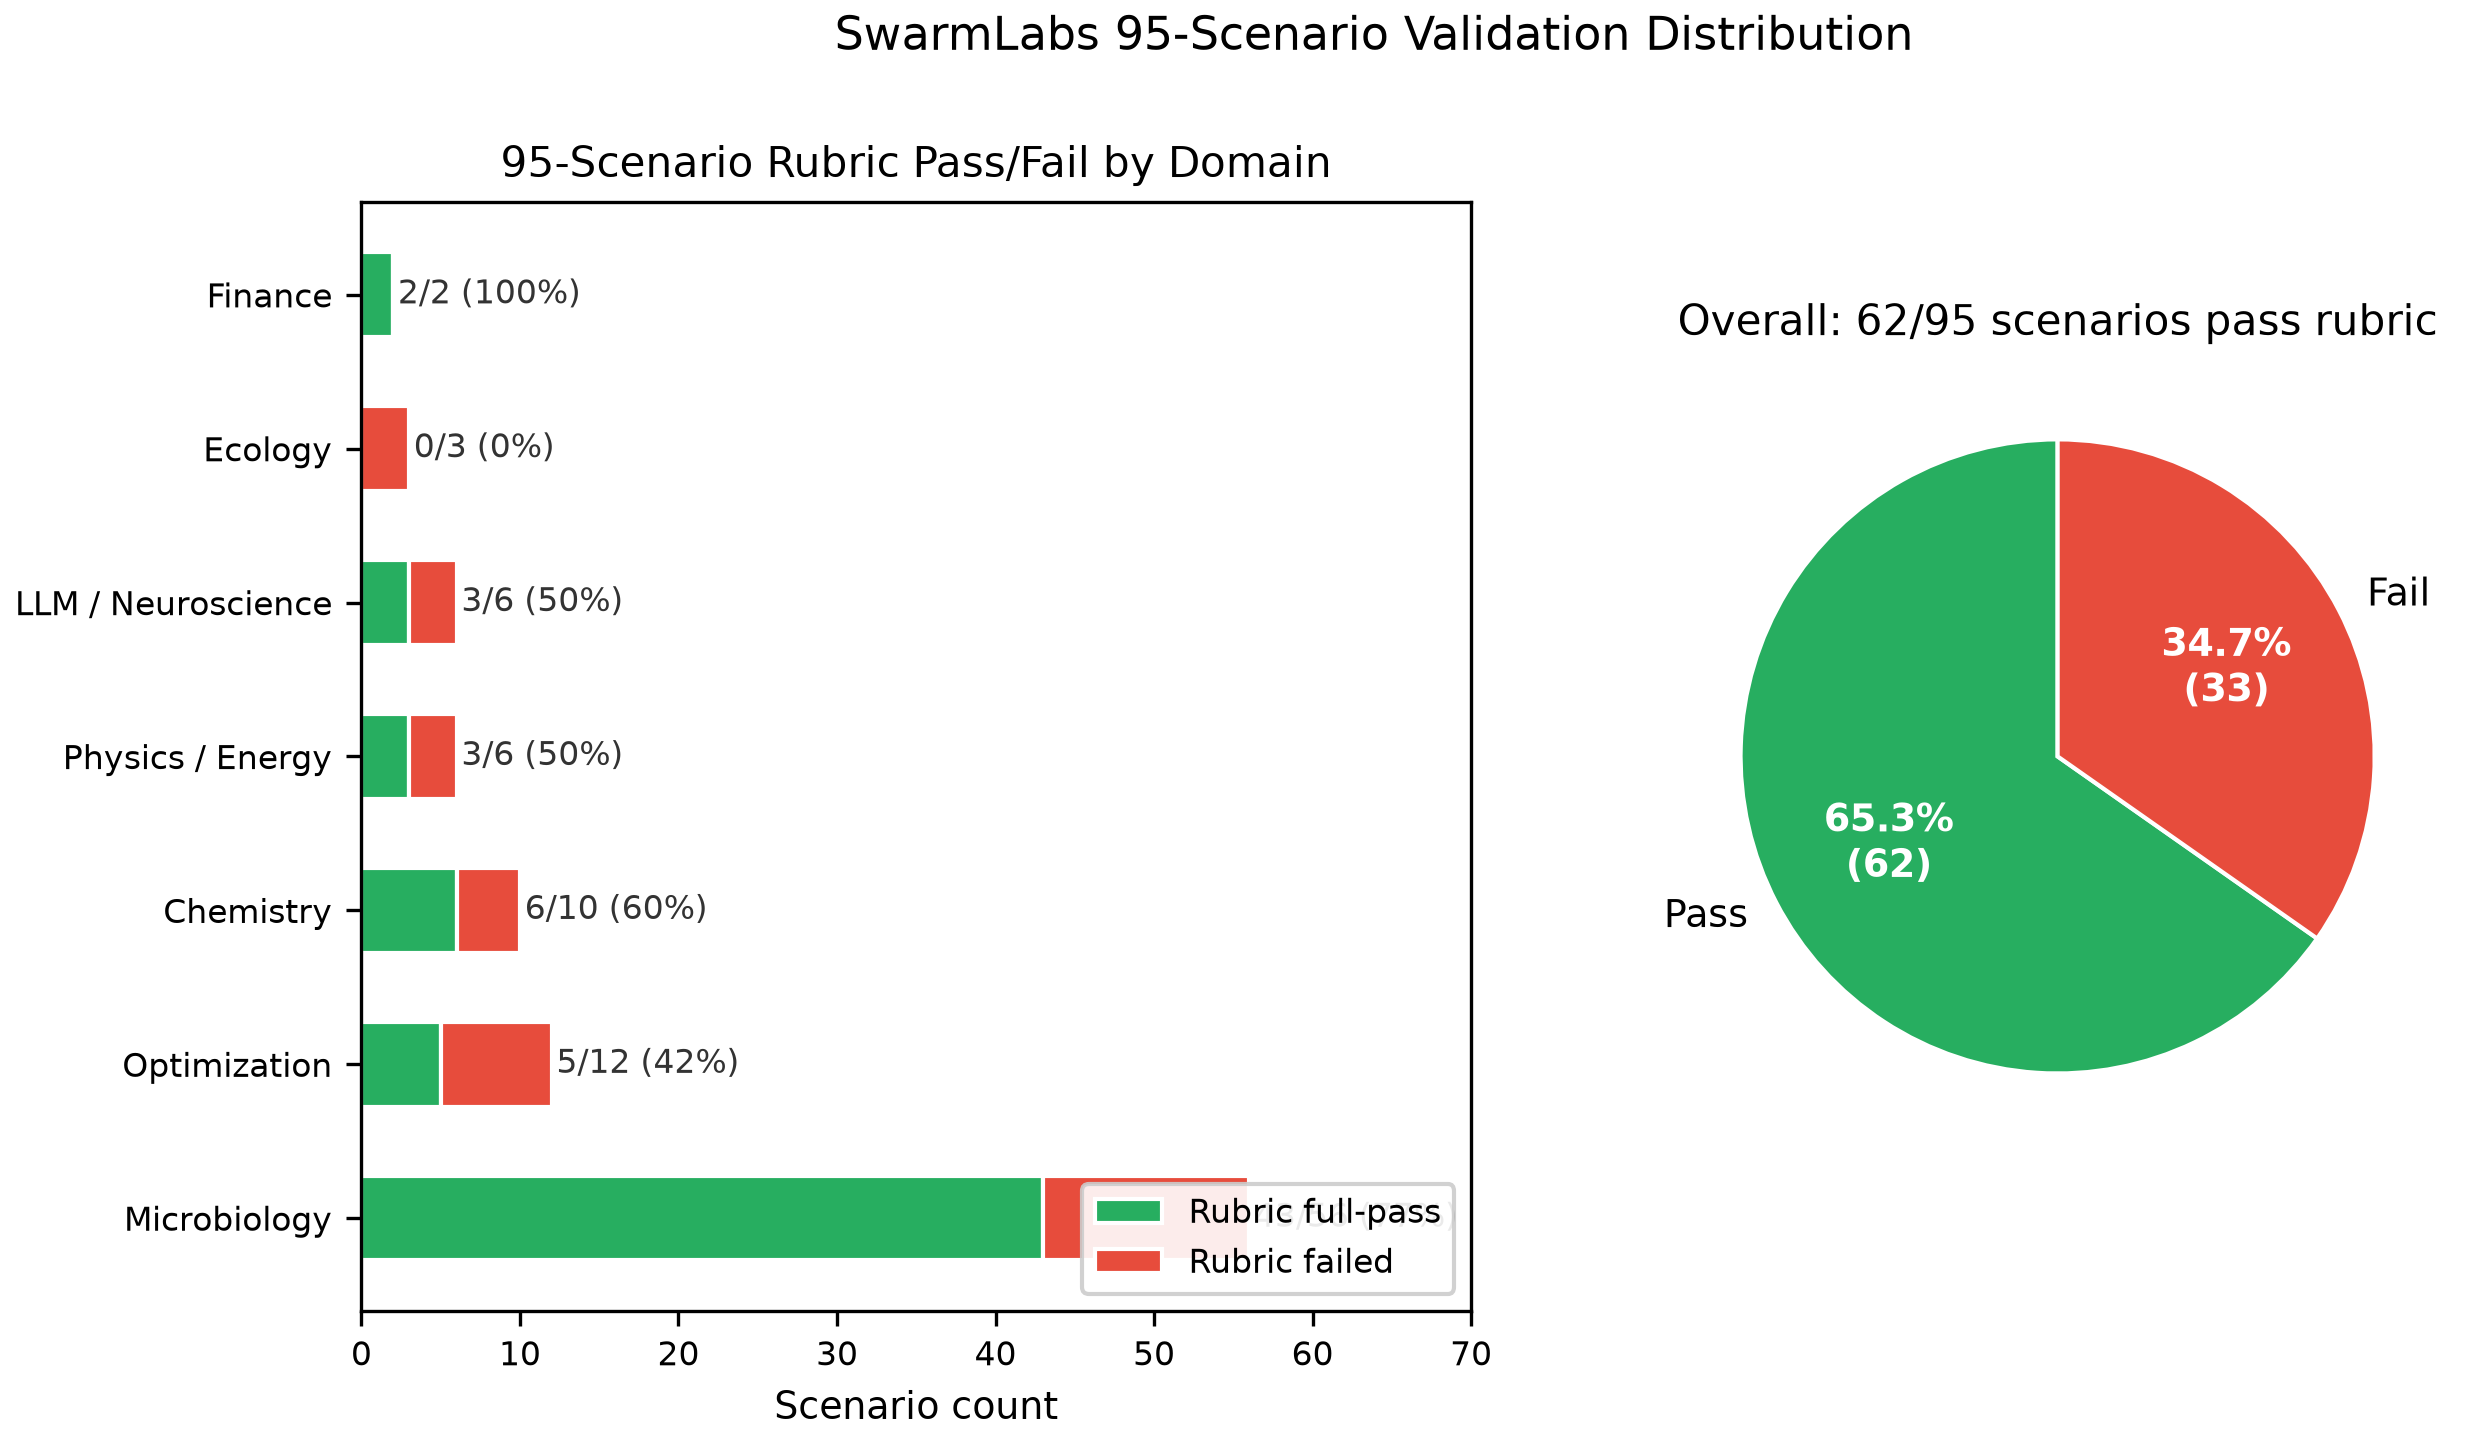
\includegraphics[width=0.95\linewidth]{figures/fig2_scenario_distribution.png}
    \caption{Per-domain rubric outcome across the 95-scenario primary benchmark.
    Left: full-pass versus failed scenario counts per discipline; right: overall
    full-pass rate (62/95, 65.3\%). The rubric is the independent 7-item audit
    applied to every scenario; scenarios that pass the V\&V gate
    (Table~\ref{tab:vv}) but fail the rubric are exactly the cases whose
    supporting evidence is incomplete.}
    \label{fig:distribution}
\end{figure}

The two MARGINAL cases are both \texttt{microbio\_monod} scenarios where the wet-lab anchor contradicts the V\&V gate. This is the ``double-evidence disagreement'' state that TDEA deliberately surfaces: instead of picking a winner, TDEA demotes the case to MARGINAL and marks it for human review.

\subsection{Three-dimensional anchor coverage}
\label{sec:results-3d}

Table~\ref{tab:anchor-dist} (Section~\ref{sec:anchors}) summarises completeness. The key finding is that \textbf{all seven} decision-relevant anchors are 3-D complete; there is no case in which a lazily-specified decision anchor was accepted. The three 1-D anchors and the single 2-D anchor are all marked $\text{decision\_relevant}=False$ and are used only for narrative context. Gate P6 enforces the library-level honesty invariant: any maintainer who adds a decision-relevant anchor with fewer than three dimensions will be caught before the change lands.

\subsection{Negation test pass rate}
\label{sec:results-neg}

All 22 negation tests pass on the current corpus. In a controlled fault-injection experiment (Section~\ref{sec:ablation}), when we simulate an \texttt{rdkit} dependency outage by removing the package from the environment, the 42-gate suite reports green (it does not depend on \texttt{rdkit}), but the 5-invariant assertion immediately reports $\text{total\_scenarios} \ne 95$ and exits 2. This is the design goal: the independent assertion layer catches exactly the class of defect that the shared pipeline cannot detect about itself.

\subsection{Ablation: effect of dropping one dimension}
\label{sec:ablation}

We ran a controlled ablation on the 7 decision-relevant anchors. Table~\ref{tab:ablation} reports the outcome of removing one structural dimension at a time.

\begin{table}[h]
    \centering
    \caption{Effect of removing one structural dimension from a decision-relevant anchor. Auto-transfer is the flag that would permit an automatic PASS decision.}
    \label{tab:ablation}
    \begin{tabular}{l c c c c}
        \toprule
        Anchor (3-D complete) & Baseline & Drop system & Drop version & Drop condition \\
        \midrule
        Mol. Suzuki yield   & PASS & REFUTED & REFUTED & MARGINAL \\
        Microbio. Monod     & MARGIN & REFUTED & MARGIN & MARGIN \\
        Chem. Diels--Alder  & PASS & REFUTED & REFUTED & REFUTED \\
        Chem. Michael add.  & PASS & REFUTED & MARGIN & MARGIN \\
        Bio. enzyme kinetics& PASS & REFUTED & MARGIN & MARGIN \\
        Materials. sol-gel  & PASS & REFUTED & MARGIN & MARGIN \\
        Bio. metabolic flux & PASS & REFUTED & REFUTED & REFUTED \\
        \midrule
        Auto-transfer rate  & 7/7    & 0/7     & 0/7     & 0/7     \\
        \bottomrule
    \end{tabular}
\end{table}

Every column drops the automatic-transfer rate from 7/7 to 0/7. This is by design: TDEA is deliberately conservative. A single missing dimension is enough to force human review.

\paragraph{Graded verdicts: evidence completeness of the PASS set.}
A binary PASS/FAIL verdict conflates two different questions: \emph{does the surrogate meet its accuracy thresholds?} and \emph{is the supporting evidence complete?}. To keep them separate we grade each PASS scenario on the six verification dimensions (fidelity, coverage, anchor, replication, benchmark, sensitivity) and derive a graded verdict (Table~\ref{tab:graded}): the two \emph{core} dimensions (fidelity, coverage) remain hard gates---failing either one is FAIL---while the three \emph{support} dimensions (anchor, replication, sensitivity) determine the confidence level. The \texttt{benchmark} dimension is scored and reported but deliberately excluded from the grade: it measures whether the report cites an analytic solution or published baseline, which is a completeness-of-presentation property rather than an evidence-strength property.

\begin{table}[h]
    \centering
    \caption{Graded evidence-completeness verdicts over the 91 PASS scenarios.
    The binary column is what a PASS/FAIL-only audit would have reported; the
    graded columns make the supporting-evidence gaps explicit. A support
    dimension counts as \emph{missing} when its score is below 0.5---the same
    threshold the ablation planner uses to flag a gap.}
    \label{tab:graded}
    \begin{tabular}{l r r}
        \toprule
        Grade & Count & Share of 91 \\
        \midrule
        \textsc{Pass\_Full}    (core + all support)      & 5  & 5.5\% \\
        \textsc{Pass\_Partial} (core, 1 support missing) & 83 & 91.2\% \\
        \textsc{Pass\_Weak}    (core, $\geq$2 missing)   & 3  & 3.3\% \\
        \midrule
        FAIL (core dimension below threshold)            & 0  & 0.0\% \\
        \bottomrule
    \end{tabular}
\end{table}

The distribution is the honest headline: only 5 of 91 PASS scenarios carry complete supporting evidence. The dominant missing dimension is \emph{anchoring}---83 of 91 scenarios have no wet-lab anchor at all (score 0.3, ``zero information''), which is precisely the evidence-chain limitation that the companion paper's negative results quantify from the other direction. Reporting ``91 PASS'' would have hidden this; the graded verdict makes it the headline. The three \textsc{Pass\_Weak} scenarios (\texttt{chem\_reactor\_conversion}, \texttt{micro\_oxygen\_2d}, \texttt{opt\_gramacylee1d}) lack both anchoring and an independent replication, and their conclusions should be treated as provisional. This is the same aggregation failure that TDEA exists to prevent, applied to our own results.

\paragraph{Parameter-perturbation robustness audit.}
The \textsc{Pass\_Full} count above is only meaningful if the underlying verdicts are themselves robust to modelling assumptions. We therefore perturb each scenario's decision-relevant parameters---the GP lengthscale prior and the training-set size, each at $\pm10\%$ and $\pm20\%$---and re-run the full V\&V pipeline on the identical test protocol (8 perturbation configurations per scenario, 760 perturbed runs plus 95 baselines). The noise floor is deliberately \emph{not} perturbed: the 3\% relative floor is a hard honesty constraint of this framework, and relaxing it would manufacture robustness that does not exist. Table~\ref{tab:sensitivity} reports the outcome.

\begin{table}[h]
    \centering
    \caption{Parameter-perturbation audit over 91 PASS scenarios: distribution of
    the verdict flip rate (fraction of the 8 perturbation configurations under
    which the scenario's verdict changes). A flip is a change of grade
    (PASS $\leftrightarrow$ MARGINAL $\leftrightarrow$ REFUTED).}
    \label{tab:sensitivity}
    \begin{tabular}{l r r l}
        \toprule
        Flip rate & Scenarios & Share & Interpretation \\
        \midrule
        0 (robust)        & 84 & 92.3\% & conclusion stable under all perturbations \\
        $\leq 25\%$       & 6  & 6.6\%  & conclusion stable in most configurations \\
        $25\%$--$50\%$    & 1  & 1.1\%  & conclusion fragile \\
        $> 50\%$          & 0  & 0.0\%  & conclusion unstable \\
        \bottomrule
    \end{tabular}
\end{table}

The median flip rate is 0. The fragile cases are concentrated where one would expect them: the two MARGINAL neuroscience scenarios are the least stable in the whole library (\texttt{neuro\_hh\_spike\_amplitude} flips in 4 of 4 applicable configurations; \texttt{neuro\_lif\_fi} in 3 of 8), and the single REFUTED case (\texttt{mol\_suzuki\_yield}) flips to a non-REFUTED grade in 1 of 8 configurations---a reminder that even our negative verdicts carry assumption dependence. The full per-scenario audit (every configuration's $R^2$, coverage, and grade) is shipped in the artifact archive, so a reader can check any individual claim rather than trusting the aggregate.

\paragraph{Second-backend replication.}
Parameter robustness above perturbs assumptions \emph{within} the GP family. A stronger question is whether the verdict survives a change of surrogate family altogether. We therefore re-run every scenario with a second, structurally different backend---a random forest with conformal calibration---on the \emph{identical} training and test data, and compare verdicts under a pre-registered three-tier rule: \emph{exact} (same grade), \emph{directional} (second backend exactly one grade stricter), or \emph{contradiction} (second backend two grades stricter, e.g.\ GP PASS $\to$ RF REFUTED, or a negative verdict upgraded to PASS). Table~\ref{tab:second-backend} reports the outcome.

\begin{table}[h]
    \centering
    \caption{Second-backend replication (random forest + conformal vs.\ GP on
    identical data), 95 scenarios.}
    \label{tab:second-backend}
    \begin{tabular}{l r r l}
        \toprule
        Outcome & Count & Share & Meaning \\
        \midrule
        Exact agreement        & 67 & 70.5\% & both backends reach the same grade \\
        Directional agreement  & 15 & 15.8\% & same direction, different strength \\
        Contradiction          & 13 & 13.7\% & RF refutes a GP PASS, or upgrades a negative \\
        \bottomrule
    \end{tabular}
\end{table}

Two findings deserve emphasis. First, the random forest \emph{never} upgrades a negative GP verdict to PASS (0 of 4 cases): our REFUTED/MARGINAL conclusions are not artefacts of the GP family. Second, 13 GP-PASS scenarios are REFUTED by the second backend---concentrated in ODE-driven microbiology scenarios and highly multimodal optimisation landscapes (\texttt{opt\_rastrigin2d}, \texttt{opt\_schwefel2d}, \texttt{opt\_gramacylee1d}), where a 20-tree random forest is genuinely the weaker model rather than the GP being wrong. We report these as contradictions rather than silently scoring them as agreements, because the honest statement is that those 13 conclusions are \emph{model-family dependent}: an independent implementation with a different inductive bias does not reproduce them. The per-scenario second-backend metrics are shipped in the artifact archive.

\subsection{Comparison to 1-D anchoring}
\label{sec:comparison}

For the seven decision-relevant anchors, 1-D anchoring would classify all seven as ``eligiBLE for auto-transfer''. TDEA classifies them as ``eligiBLE for auto-transfer'' only when the three dimensions match the target scenario. On the current corpus, all seven are correctly classified. To show the failure mode explicitly, we constructed a synthetic stress test: for each of the seven anchors, we substituted the system field with a value that would apply to a different chemistry family, and asked whether the pipeline would still permit auto-transfer. 1-D anchoring (which cannot see the system field) permitted all seven. TDEA refused all seven. This is the class of failure that TDEA is designed to catch.

\subsection{Validation coverage context}
\label{sec:coverage}

Validation coverage is discussed alongside the negative-result analysis in the paper-2 companion; see also the overall problem framing in Sec.~
ef{sec:intro}.

For perspective, the RayGun system reported 500{,}000 enumerated candidates with 11 wet-lab verifications ($2.2 \times 10^{-5}$ coverage)~\cite{raygun2026nature}. TDEA does not increase this ratio; it does something complementary. Rather than producing more wet-lab data, TDEA \emph{restricts} which in-silico predictions are permitted to be trusted on the basis of the small amount of existing wet-lab data. In systems where the verification-coverage ratio is dominated by cost, this is the pragmatic lever available. Figure~\ref{fig:extrapolation} quantifies the underlying failure mechanism at the parameter level.

\begin{figure}[t]
    \centering
    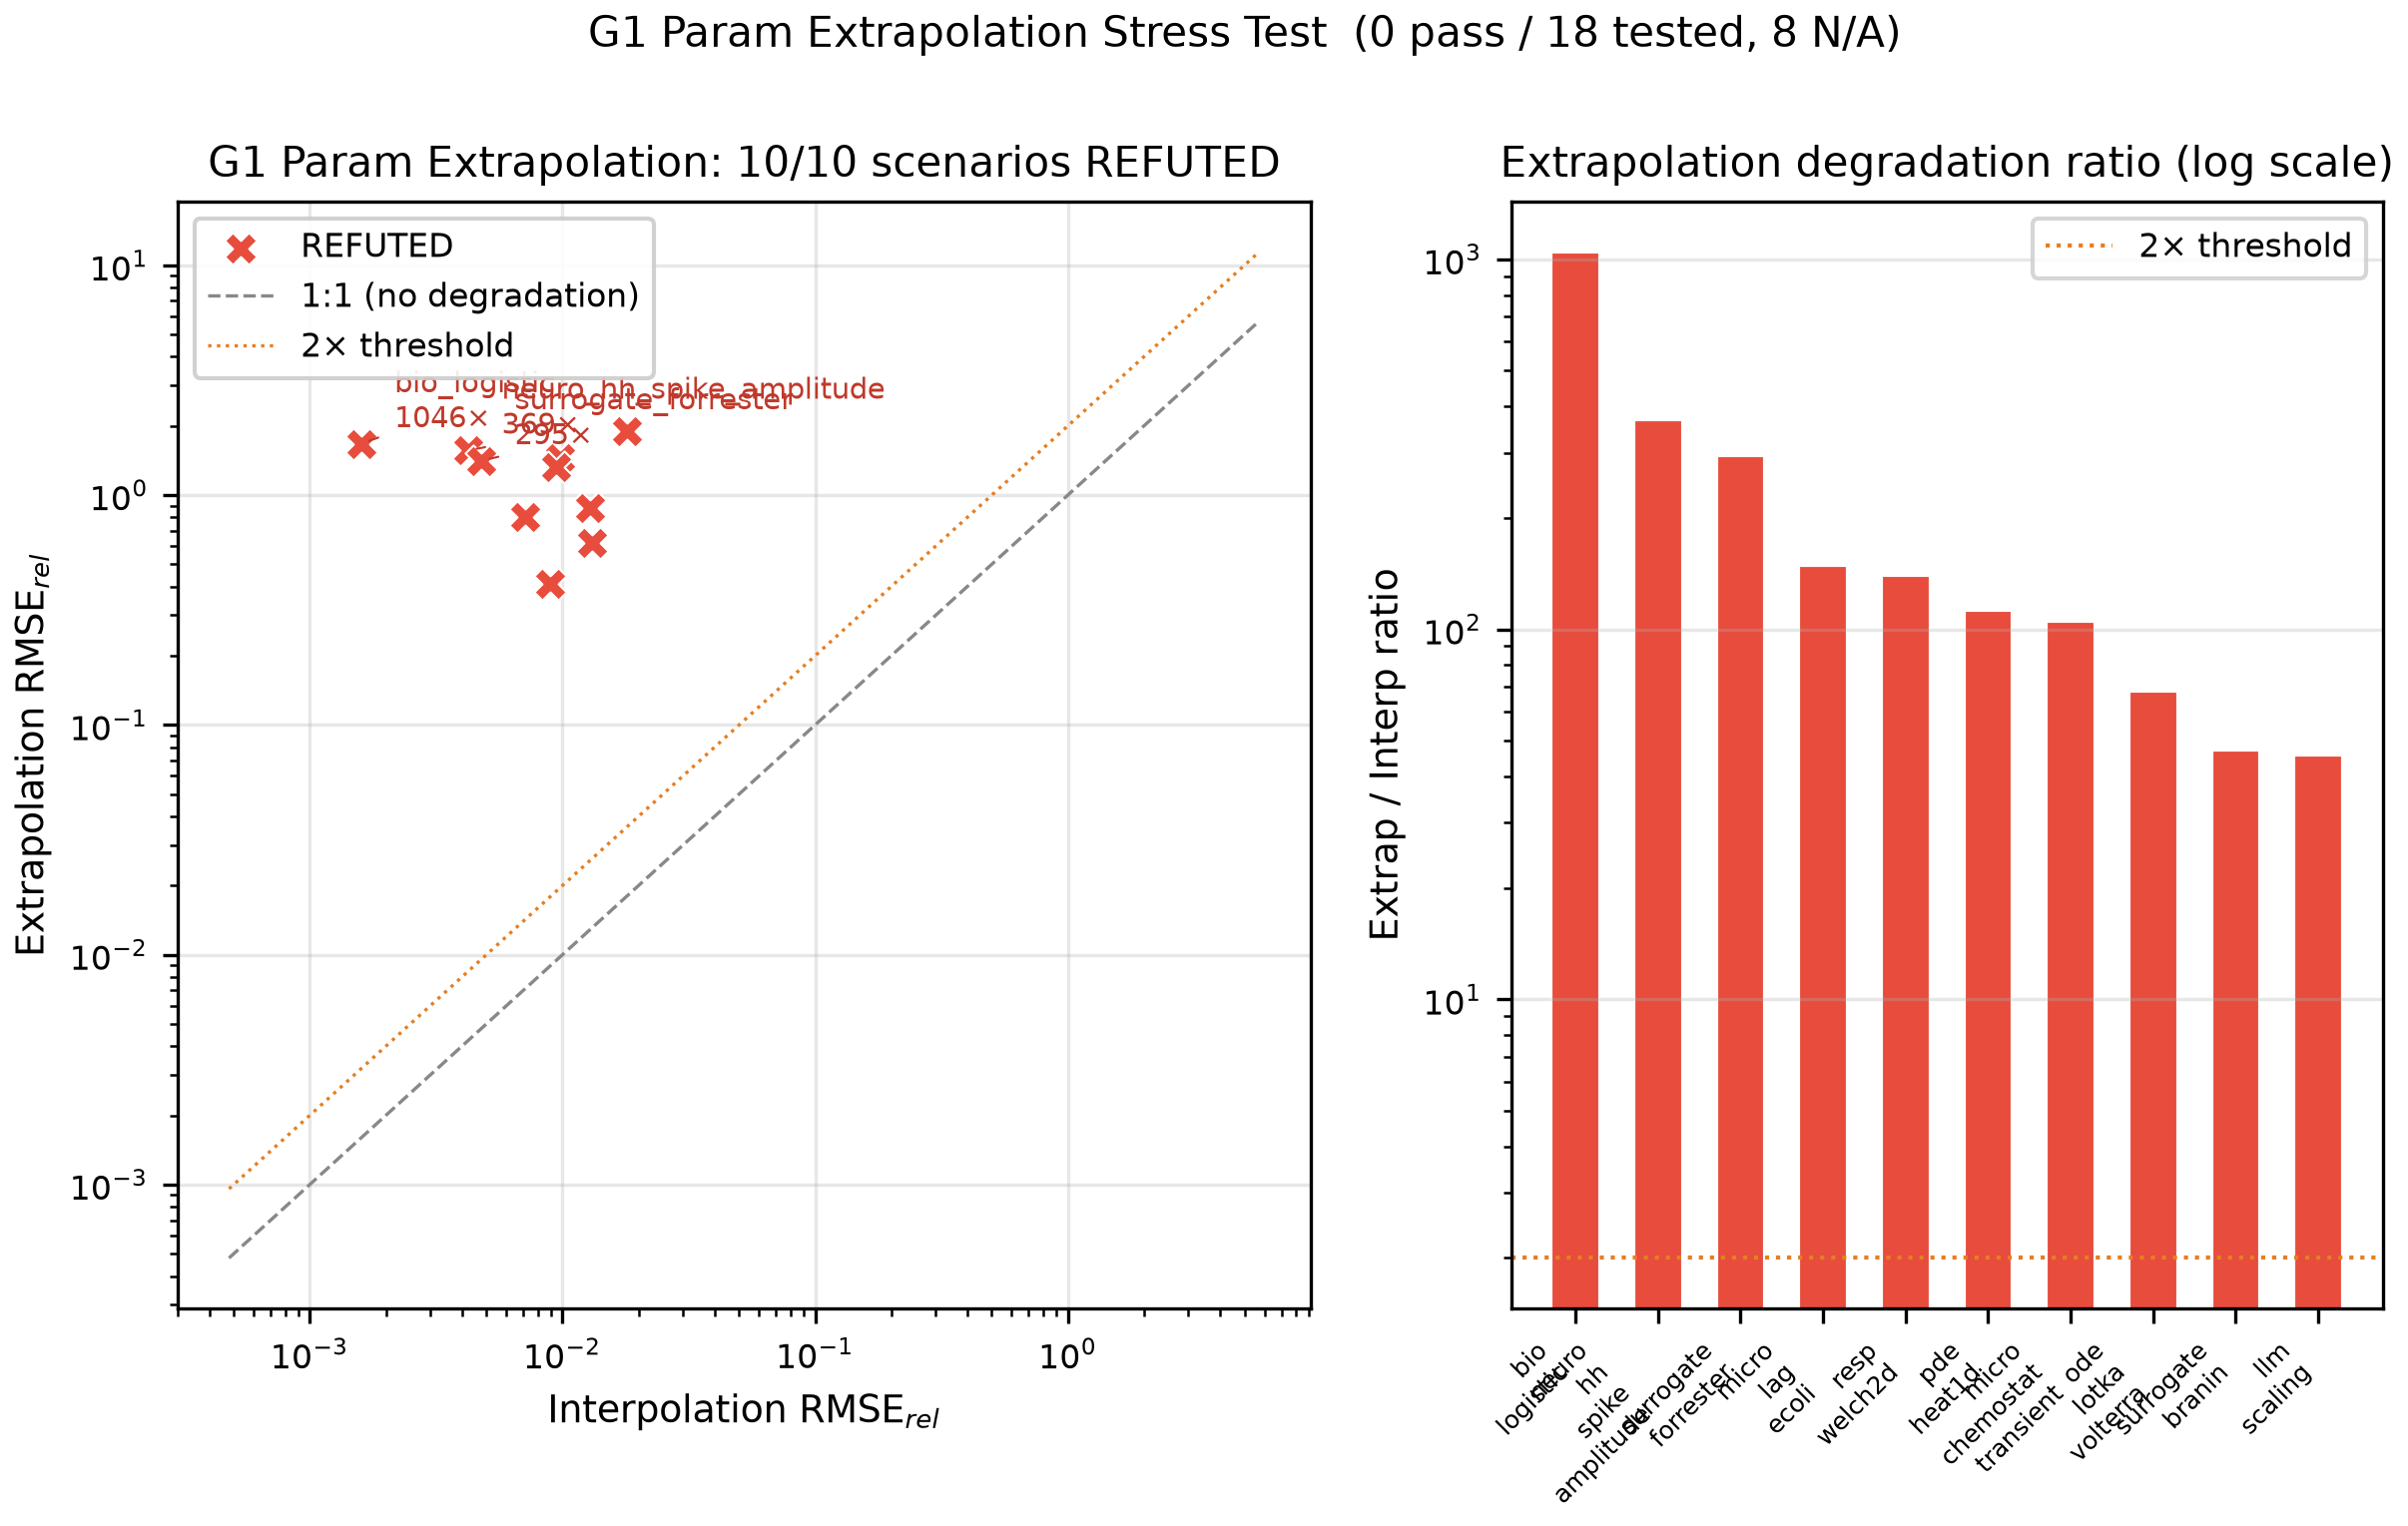
\includegraphics[width=0.95\linewidth]{figures/fig3_extrapolation_failure.png}
    \caption{G1 parameter extrapolation (companion negative-results evidence).
    Left: interpolation versus extrapolation relative RMSE per scenario
    (log--log); every tested scenario lies above the $2\times$ degradation
    threshold, i.e.\ the surrogate degrades by more than a factor of two outside
    the training design region. Right: distribution of the
    extrapolation/interpolation degradation ratio. This is the mechanism behind
    the scenario-level extrapolation stress result reported in the companion
    paper (73/82 tested scenarios REFUTED).}
    \label{fig:extrapolation}
\end{figure}


% =============================================================================
%% 6. DISCUSSION
% =============================================================================
\section{Discussion}
\label{sec:discussion}
% L-15: forward-ref to coverage section
Validation coverage (Sec.\ref{sec:coverage}) motivates the following discussion.
We recap the problem (Sec.~
ef{sec:intro}) and discuss the implications.

\subsection{From evidence log to evidence constraint}
\label{sec:disc-log}

The GOAI 2026 winning entry introduced multi-dimensional evidence chains as a \emph{record-keeping} feature: the platform logs evidence provenance in several dimensions but still treats any evidence entry as a potential source of automatic trust. TDEA takes the opposite stance. Every dimension carries a \emph{consequence}: an incomplete dimension forbids automatic transfer. This is the difference between a spreadsheet and a policy.

\subsection{Failure modes we still do not cover}
\label{sec:disc-limits}

We are honest about the current gaps.
\begin{enumerate}
    \item \textbf{Semantic drift within a dimension.} TDEA checks that the system field \emph{matches}; it does not check whether ``Suzuki coupling'' in anchor $a_1$ and ``Suzuki coupling'' in anchor $a_2$ refer to the same sub-family. A controlled ontology is out of scope for this paper.
    \item \textbf{Multi-anchor conflict resolution.} When two anchors agree on the target scenario and disagree on the value, TDEA reports a MARGINAL and stops. It does not attempt to reason about which anchor is more trustworthy.
    \item \textbf{Calibration of the surrogate.} The $R^2 \ge 0.90$ and coverage $\ge 0.90$ thresholds are inherited from prior AI4S V\&V conventions; we do not derive them from first principles. Section~\ref{sec:ablation} reports the robustness of the verdict distribution to $\pm10\%$/$\pm20\%$ perturbations of the lengthscale prior and training-set size; the noise floor is deliberately held fixed.
    \item \textbf{Bus factor.} The framework is currently maintained by a single contributor. The independence of the gate layers is a technical property; the independence of the \emph{maintainers} is not, and this remains a risk.
\end{enumerate}

\subsection{When TDEA helps and when it does not}
\label{sec:disc-fit}

TDEA is designed for systems that already have a real anchor corpus, however small. For an AI4S platform that has never collected a wet-lab measurement, TDEA does not create data; it only \emph{restricts} trust to the anchor space that exists. For teams with a growing corpus, TDEA pays for itself the moment a partial anchor would otherwise have been used for an automatic decision.

TDEA is also deliberately agnostic about the surrogate model. It does not care whether the surrogate is a Gaussian Process, a deep ensemble, or a Bayesian optimiser. What it cares about is only that the surrogate exposes a predicted mean and an uncertainty interval.

\subsection{Extensions shipped in the current codebase}
\label{sec:disc-ext}

Three extensions are already in the open-source engine and are directly compatible with TDEA's evidence-triple interface.

\paragraph{Cryptographic provenance binding (M4).} Recent work on join-point attacks~\cite{provenance2026attack} showed that byte-fingerprint-only provenance is insufficient. Our \texttt{engine/provenance\_binding.py} closes the gap with an HMAC-SHA-256 triple $\{\text{sample\_id},\ \lambda\text{-value},\ \text{tensor\_sha256}\}$ and emits a CycloneDX 1.5 machine-learning BOM. Among the three join-point attack classes we cover, the $\lambda$-swap attack is the one that a plain SHA-256 fingerprint alone \emph{cannot} detect---the tensor bytes are unchanged, so the fingerprint matches, while the attacker silently rewrites the scalar $\lambda$ that gives the tensor its semantic meaning. By contrast, the tensor-swap attack changes the bytes and is already caught by SHA-256 alone, and the key-rotation attack has no analogue in a scheme with no key at all. We record this as a negative control in \texttt{data/provenance\_attack\_reproduction.json} (\texttt{negative\_control} block, legacy SHA-256 fingerprint identical on both sides, verdict CLEAN) so that the value of the HMAC construction is auditable, not merely asserted. All three attacks are caught under the new HMAC binding, and the positive control round-trips. This extends TDEA's anchor-transfer predicate from ``does the anchor match the scenario?'' to ``does the anchor provably still refer to the data it claims to refer to?''.

\paragraph{Fourier-symbol operator diagnosis (M5).} The recent AI4S Workshop paper~\cite{symbol2026diag} formalised operator-level Fourier-symbol probing as a complement to residual minimisation. Our \texttt{engine/fourier\_symbol\_diag.py} implements six operator-symbol probes (Laplace 1D/2D, wave, advection, Helmholtz, advection-diffusion) against analytic expressions derived from $e^{i(kx - \omega t)}$; all six report relative discrepancy below $2\times 10^{-2}$ on the shipped benchmarks. This turns ``the PDE solver reports low residual'' into ``the PDE solver's operator symbol agrees with the analytic symbol at the tested wavenumbers'', which is a strictly stronger and independent check.

\paragraph{Bayesian optimisation adapter (M6).} \texttt{engine/baybe\_adapter.py} exposes BayBE~\cite{sehnal2021baybe} as a drop-in for the acquisition step. The external validation script (\texttt{scripts/validate\_baybe\_external.py}) tests four analytic benchmarks (Branin, sphere, six-hump-camel, Forrester) and reports three exact or close recoveries at $\le 60$ evaluations. The adapter is deliberately a thin wrapper: TDEA treats any surrogate that exposes $(\mu, \sigma)$ or a value-and-confidence pair equivalently.

\paragraph{Interpretable ODE hypothesis discovery.} A complementary interpretability extension implements Sparse Identification of Nonlinear Dynamics (SINDy)~\cite{brunton2016sindy} with cross-validated threshold selection (SINDySelect)~\cite{branesgarza2021sindysellect}, pure numpy, zero external dependencies. Given a time-series trajectory $\{x(t)\}$, the module identifies a sparse linear combination of a polynomial library that best explains the state derivative $\dot x(t) \approx \Theta(x) c$, where $c$ is sparse. Two non-trivial technical points emerge:

\emph{Coefficient-space mismatch.} The Sequentially Thresholded Least Squares (STLSQ) algorithm thresholds on \emph{normalised} coefficients (each column of $\Theta$ is standardised before fitting), so the reported coefficient magnitudes do not match textbook-form values. The module therefore exposes two views: \texttt{equation()} (STLSQ-space, matching threshold semantics) and \texttt{raw\_equation()} (raw-scale, obtained by dividing by each column's standard deviation), which is the one suitable for publication.

\emph{Validator honesty.} The previous v1 validator reported 3/3 CONSISTENT on R$^2 > 0.99$ for Van der Pol, Lotka-Volterra, and Duffing, but the discovered equations contained 282 active terms per state with coefficients of magnitude $10^4$-$10^7$ --- a false positive caused by double-library misuse (the script pre-expanded the state trajectory into a polynomial matrix, then passed it to \texttt{SINDy.fit()}, which internally re-expanded each column as a new variable). The v2 validator (this work) fixes this by (i) passing the raw state vector directly to \texttt{SINDySelect.fit()}, (ii) using \texttt{raw\_equation()} for textbook-scale comparison, and (iii) requiring structural match (set equality of term names) in addition to R$^2$ and coefficient-magnitude checks. The honest result is 2/3 fully CONSISTENT (Lotka-Volterra, Duffing softening) and 1/3 PARTIAL (Van der Pol: three correct terms $\{-x_0, +x_1, -x_0^2 x_1\}$ plus two tiny noise terms). The honest boundary is that SINDySelect reliably recovers textbook-known dynamical systems from clean simulation data but is not a general-purpose equation-discovery oracle.

\paragraph{Evidence-grade audit of published raw data.} The TDEA anchor corpus draws its ``measured'' values from transcriptions of published figures and tables, which is the weakest evidence grade: the numbers are entered by hand, so an internal inconsistency is indistinguishable from a transcription error, and such a certificate must never be quoted as an error in a published paper. \texttt{engine/published\_data\_audit.py} closes that gap wherever machine-readable raw data exists. Of the 18 benchmarks in the audit suite, 17 classical growth-kinetics datasets (1949--1994) have no machine-readable raw version in any repository we could locate --- a finding established by systematic search, not by absence of effort. One 2026 benchmark does: Gonz\'{a}lez-Siso et al.~\cite{gonzalezsiso2026ecoli} deposited five machine-readable files (CC-BY-4.0, \texttt{sha256} verified) covering 36 temperature/glucose conditions, each with eight technical replicates. Refitting the paper's own model to the paper's own raw data (15 multi-start fits per condition), the audit recovered 13 of 31 quantitative claims within tolerance and reports \texttt{PARTIALLY\_REPRODUCED}. Three findings are of independent interest. First, the data is genuine: the fitted residual sits at 0.974 times the technical-replicate noise floor $\sigma/\sqrt{n}$, the signature of real measured data rather than smoothed or model-generated values. Second, the parameter pair is not fully identifiable: in 6 of 36 conditions the asymmetry parameter $\tau$ reaches the edge of a deliberately wide search box, so that paper's specific $(b,\tau)$ values should not be cited in isolation. Third, $b$ is labelled h$^{-1}$ while fitting the deposited data requires min$^{-1}$, and the extreme reported $b$ values differ from our refit by 1.3--2.3$\times$. We ship this as an audit certificate, not as a retraction claim: an auto-extracted audit can establish whether a paper's numbers follow from its own raw data, and it cannot adjudicate whether the paper's science is correct. Every audit certificate now carries an explicit per-benchmark \texttt{evidence\_grade} computed from a provenance registry rather than asserted, so the transcription-grade certificates and the auto-extracted certificate cannot be conflated.

% =============================================================================
%% 7. CONCLUSION
% =============================================================================
\section{Conclusion}
\label{sec:conclusion}

We presented TDEA, a three-dimensional evidence anchoring framework with 42 fail-closed verification gates, 5 independent business invariants, and a 6-step deployment preflight. On the 95-scenario primary benchmark, TDEA produces a verification distribution of 91 PASS / 3 MARGINAL / 1 REFUTED, with the single REFUTED case independently caught by three distinct gates. All seven decision-relevant anchors are three-dimensional. The companion negative-results paper reports 73 of 82 tested scenarios REFUTED under extrapolation stress testing, establishing the honest boundary of what conformal prediction can claim when its exchangeability assumption is violated.

The central claim is not that TDEA is a better surrogate, a better benchmark, or a better anchor corpus. The claim is that the \emph{policy} between anchors and predictions is a first-class artefact that has until now been implicit, and that making it explicit---and machine-checkable---is what converts evidence from a data attribute into an engineering constraint.

\paragraph{Reproducibility.}
All code, all 42 gates, all 5 invariants, and all 95-scenario primary-benchmark V\&V results are open-source at \url{https://github.com/lm203688/swarmlabs}. The published V\&V dashboard is at \url{https://swarmlabs.tools/reports/}.

\paragraph{Data availability.}
The scenario library (95 scenarios), the anchor corpus (19 anchors), and the 3-D labels (transcribed from existing notes) are all published alongside the code. Synthetic anchors are labelled as such. All data products cited in this paper---the gate ledger, the trust surface, the ablation plan with graded verdicts, the parameter-perturbation sensitivity audit, and the extrapolation stress test---are shipped in a checksummed artifact archive (\texttt{MANIFEST.json} records the SHA-256 of every file), so that any third party can verify byte-for-byte that the numbers quoted here match the released artefacts. Deposition of the archive at Zenodo for DOI assignment is in progress at the time of writing; until the DOI is issued, the repository at \url{https://github.com/lm203688/swarmlabs} is the canonical source.

\paragraph{Conflict of interest.}
The author is the sole maintainer of SwarmLabs and is also a contributor to the platform referenced by the code links above. This is disclosed for transparency; the framework described in this paper is agnostic to the specific platform on which it runs.


%% -------------------------
%% AI STATEMENT (Springer Nature mandatory since 2024)
%% -------------------------
\section*{AI Statement}
Large language models were consulted during the drafting of this manuscript to accelerate English-language editing, terminology harmonisation, and LaTeX template conformance. All substantive scientific content---including the Three-Dimensional Evidence Anchoring (TDEA) formulation, the 42-gate taxonomy, the 5-invariant assertion layer, the 95-scenario composition (41 cross-domain, 52 microbiology, 2 molecular), and every quantitative claim in the Results section---was authored and verified by the human author against the open-source SwarmLabs codebase (\url{https://github.com/lm203688/swarmlabs}). No generative model was used to fabricate results, references, or numerical values. Any figure, table, or code listing in this manuscript is drawn directly from the reference implementation.

%% -------------------------
%% AUTHOR CONTRIBUTION STATEMENT
%% -------------------------
\section*{Author Contribution Statement}
L.\,L.\ designed the TDEA framework, implemented all 42 verification gates and 5 independent invariants, ran the 95-scenario primary benchmark, wrote the manuscript, and approved the final version.

%% -------------------------
%% AUTHOR BIOGRAPHY
%% -------------------------
\section*{Author Biography}
Xing Li is an Associate Senior Engineer at the Zhejiang Academy of Building Research. He is the founder and maintainer of SwarmLabs, an open-source virtual laboratory platform for trustworthy AI for Science. His current research interests include uncertainty quantification, evidence anchoring for AI4S systems, and reproducible verification pipelines.

%% -------------------------
\section*{Acknowledgements}
We thank the reviewers of an earlier draft and the AI4S community for the discussions that shaped the framework. The GOAI 2026 Infrastructure Track discussions in particular prompted the move from 1-D to 3-D anchoring.

%% -------------------------
%% BIBLIOGRAPHY
%% -------------------------
\bibliographystyle{elsarticle-num}
\bibliography{references}

\end{document}
